% Options for packages loaded elsewhere
\PassOptionsToPackage{unicode}{hyperref}
\PassOptionsToPackage{hyphens}{url}
\documentclass[
]{article}
\usepackage{xcolor}
\usepackage[margin=1in]{geometry}
\usepackage{amsmath,amssymb}
\setcounter{secnumdepth}{-\maxdimen} % remove section numbering
\usepackage{iftex}
\ifPDFTeX
  \usepackage[T1]{fontenc}
  \usepackage[utf8]{inputenc}
  \usepackage{textcomp} % provide euro and other symbols
\else % if luatex or xetex
  \usepackage{unicode-math} % this also loads fontspec
  \defaultfontfeatures{Scale=MatchLowercase}
  \defaultfontfeatures[\rmfamily]{Ligatures=TeX,Scale=1}
\fi
\usepackage{lmodern}
\ifPDFTeX\else
  % xetex/luatex font selection
\fi
% Use upquote if available, for straight quotes in verbatim environments
\IfFileExists{upquote.sty}{\usepackage{upquote}}{}
\IfFileExists{microtype.sty}{% use microtype if available
  \usepackage[]{microtype}
  \UseMicrotypeSet[protrusion]{basicmath} % disable protrusion for tt fonts
}{}
\makeatletter
\@ifundefined{KOMAClassName}{% if non-KOMA class
  \IfFileExists{parskip.sty}{%
    \usepackage{parskip}
  }{% else
    \setlength{\parindent}{0pt}
    \setlength{\parskip}{6pt plus 2pt minus 1pt}}
}{% if KOMA class
  \KOMAoptions{parskip=half}}
\makeatother
\usepackage{color}
\usepackage{fancyvrb}
\newcommand{\VerbBar}{|}
\newcommand{\VERB}{\Verb[commandchars=\\\{\}]}
\DefineVerbatimEnvironment{Highlighting}{Verbatim}{commandchars=\\\{\}}
% Add ',fontsize=\small' for more characters per line
\usepackage{framed}
\definecolor{shadecolor}{RGB}{248,248,248}
\newenvironment{Shaded}{\begin{snugshade}}{\end{snugshade}}
\newcommand{\AlertTok}[1]{\textcolor[rgb]{0.94,0.16,0.16}{#1}}
\newcommand{\AnnotationTok}[1]{\textcolor[rgb]{0.56,0.35,0.01}{\textbf{\textit{#1}}}}
\newcommand{\AttributeTok}[1]{\textcolor[rgb]{0.13,0.29,0.53}{#1}}
\newcommand{\BaseNTok}[1]{\textcolor[rgb]{0.00,0.00,0.81}{#1}}
\newcommand{\BuiltInTok}[1]{#1}
\newcommand{\CharTok}[1]{\textcolor[rgb]{0.31,0.60,0.02}{#1}}
\newcommand{\CommentTok}[1]{\textcolor[rgb]{0.56,0.35,0.01}{\textit{#1}}}
\newcommand{\CommentVarTok}[1]{\textcolor[rgb]{0.56,0.35,0.01}{\textbf{\textit{#1}}}}
\newcommand{\ConstantTok}[1]{\textcolor[rgb]{0.56,0.35,0.01}{#1}}
\newcommand{\ControlFlowTok}[1]{\textcolor[rgb]{0.13,0.29,0.53}{\textbf{#1}}}
\newcommand{\DataTypeTok}[1]{\textcolor[rgb]{0.13,0.29,0.53}{#1}}
\newcommand{\DecValTok}[1]{\textcolor[rgb]{0.00,0.00,0.81}{#1}}
\newcommand{\DocumentationTok}[1]{\textcolor[rgb]{0.56,0.35,0.01}{\textbf{\textit{#1}}}}
\newcommand{\ErrorTok}[1]{\textcolor[rgb]{0.64,0.00,0.00}{\textbf{#1}}}
\newcommand{\ExtensionTok}[1]{#1}
\newcommand{\FloatTok}[1]{\textcolor[rgb]{0.00,0.00,0.81}{#1}}
\newcommand{\FunctionTok}[1]{\textcolor[rgb]{0.13,0.29,0.53}{\textbf{#1}}}
\newcommand{\ImportTok}[1]{#1}
\newcommand{\InformationTok}[1]{\textcolor[rgb]{0.56,0.35,0.01}{\textbf{\textit{#1}}}}
\newcommand{\KeywordTok}[1]{\textcolor[rgb]{0.13,0.29,0.53}{\textbf{#1}}}
\newcommand{\NormalTok}[1]{#1}
\newcommand{\OperatorTok}[1]{\textcolor[rgb]{0.81,0.36,0.00}{\textbf{#1}}}
\newcommand{\OtherTok}[1]{\textcolor[rgb]{0.56,0.35,0.01}{#1}}
\newcommand{\PreprocessorTok}[1]{\textcolor[rgb]{0.56,0.35,0.01}{\textit{#1}}}
\newcommand{\RegionMarkerTok}[1]{#1}
\newcommand{\SpecialCharTok}[1]{\textcolor[rgb]{0.81,0.36,0.00}{\textbf{#1}}}
\newcommand{\SpecialStringTok}[1]{\textcolor[rgb]{0.31,0.60,0.02}{#1}}
\newcommand{\StringTok}[1]{\textcolor[rgb]{0.31,0.60,0.02}{#1}}
\newcommand{\VariableTok}[1]{\textcolor[rgb]{0.00,0.00,0.00}{#1}}
\newcommand{\VerbatimStringTok}[1]{\textcolor[rgb]{0.31,0.60,0.02}{#1}}
\newcommand{\WarningTok}[1]{\textcolor[rgb]{0.56,0.35,0.01}{\textbf{\textit{#1}}}}
\usepackage{graphicx}
\makeatletter
\newsavebox\pandoc@box
\newcommand*\pandocbounded[1]{% scales image to fit in text height/width
  \sbox\pandoc@box{#1}%
  \Gscale@div\@tempa{\textheight}{\dimexpr\ht\pandoc@box+\dp\pandoc@box\relax}%
  \Gscale@div\@tempb{\linewidth}{\wd\pandoc@box}%
  \ifdim\@tempb\p@<\@tempa\p@\let\@tempa\@tempb\fi% select the smaller of both
  \ifdim\@tempa\p@<\p@\scalebox{\@tempa}{\usebox\pandoc@box}%
  \else\usebox{\pandoc@box}%
  \fi%
}
% Set default figure placement to htbp
\def\fps@figure{htbp}
\makeatother
\setlength{\emergencystretch}{3em} % prevent overfull lines
\providecommand{\tightlist}{%
  \setlength{\itemsep}{0pt}\setlength{\parskip}{0pt}}
\usepackage{bookmark}
\IfFileExists{xurl.sty}{\usepackage{xurl}}{} % add URL line breaks if available
\urlstyle{same}
\hypersetup{
  pdftitle={Danny Pan- HW3},
  hidelinks,
  pdfcreator={LaTeX via pandoc}}

\title{Danny Pan- HW3}
\author{}
\date{\vspace{-2.5em}}

\begin{document}
\maketitle

\begin{Shaded}
\begin{Highlighting}[]
\FunctionTok{library}\NormalTok{(tidyverse)}
\end{Highlighting}
\end{Shaded}

\begin{verbatim}
## -- Attaching core tidyverse packages ------------------------ tidyverse 2.0.0 --
## v dplyr     1.2.1     v readr     2.2.0
## v forcats   1.0.1     v stringr   1.6.0
## v ggplot2   4.0.3     v tibble    3.3.1
## v lubridate 1.9.5     v tidyr     1.3.2
## v purrr     1.2.2     
## -- Conflicts ------------------------------------------ tidyverse_conflicts() --
## x dplyr::filter() masks stats::filter()
## x dplyr::lag()    masks stats::lag()
## i Use the conflicted package (<http://conflicted.r-lib.org/>) to force all conflicts to become errors
\end{verbatim}

\begin{Shaded}
\begin{Highlighting}[]
\FunctionTok{library}\NormalTok{(MatchIt)}
\NormalTok{df\_read }\OtherTok{\textless{}{-}} \FunctionTok{read\_csv}\NormalTok{(}\StringTok{"pm25\_data.csv"}\NormalTok{)}
\end{Highlighting}
\end{Shaded}

\begin{verbatim}
## Rows: 2557 Columns: 5
## -- Column specification --------------------------------------------------------
## Delimiter: ","
## chr  (1): above
## dbl  (3): death, temp, pm25
## date (1): date
## 
## i Use `spec()` to retrieve the full column specification for this data.
## i Specify the column types or set `show_col_types = FALSE` to quiet this message.
\end{verbatim}

\begin{enumerate}
\def\labelenumi{\arabic{enumi}.}
\tightlist
\item
\end{enumerate}

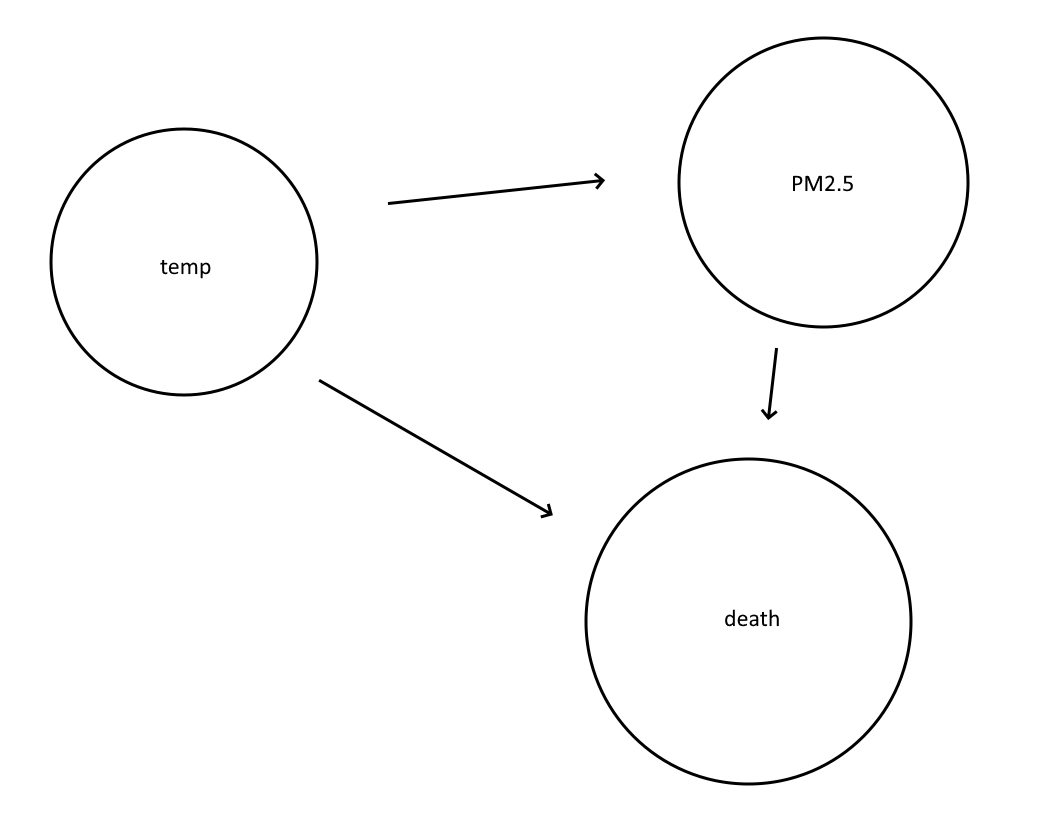
\includegraphics[width=3.69792in,height=\textheight,keepaspectratio]{images/clipboard-2880636116.png}

\begin{enumerate}
\def\labelenumi{\arabic{enumi}.}
\setcounter{enumi}{1}
\tightlist
\item
\end{enumerate}

\begin{Shaded}
\begin{Highlighting}[]
\NormalTok{df }\OtherTok{\textless{}{-}}\NormalTok{ df\_read }\SpecialCharTok{\%\textgreater{}\%} \FunctionTok{drop\_na}\NormalTok{() }\SpecialCharTok{\%\textgreater{}\%} \FunctionTok{mutate}\NormalTok{(}\AttributeTok{above =} \FunctionTok{as.integer}\NormalTok{(above }\SpecialCharTok{==} \StringTok{"above"}\NormalTok{))}

\NormalTok{ps\_model }\OtherTok{\textless{}{-}} \FunctionTok{matchit}\NormalTok{(above }\SpecialCharTok{\textasciitilde{}}\NormalTok{ temp,}
                    \AttributeTok{data =}\NormalTok{ df,}
                    \AttributeTok{method =} \StringTok{"nearest"}\NormalTok{,}
                    \AttributeTok{distance =} \StringTok{"glm"}\NormalTok{,}
                    \AttributeTok{replace =} \ConstantTok{TRUE}\NormalTok{)}

\FunctionTok{print}\NormalTok{(ps\_model)}
\end{Highlighting}
\end{Shaded}

\begin{verbatim}
## A `matchit` object
##  - method: 1:1 nearest neighbor matching with replacement
##  - distance: Propensity score
##              - estimated with logistic regression
##  - number of obs.: 2305 (original), 149 (matched)
##  - target estimand: ATT
##  - covariates: temp
\end{verbatim}

\begin{Shaded}
\begin{Highlighting}[]
\FunctionTok{summary}\NormalTok{(ps\_model)}
\end{Highlighting}
\end{Shaded}

\begin{verbatim}
## 
## Call:
## matchit(formula = above ~ temp, data = df, method = "nearest", 
##     distance = "glm", replace = TRUE)
## 
## Summary of Balance for All Data:
##          Means Treated Means Control Std. Mean Diff. Var. Ratio eCDF Mean
## distance        0.0617        0.0329          0.7464     2.3950    0.1682
## temp           67.7350       55.1391          0.6743     1.2398    0.1682
##          eCDF Max
## distance   0.4108
## temp       0.4108
## 
## Summary of Balance for Matched Data:
##          Means Treated Means Control Std. Mean Diff. Var. Ratio eCDF Mean
## distance        0.0617        0.0619         -0.0039     0.9833    0.0002
## temp           67.7350       67.7607         -0.0014     0.9941    0.0002
##          eCDF Max Std. Pair Dist.
## distance   0.0256          0.0039
## temp       0.0256          0.0014
## 
## Sample Sizes:
##               Control Treated
## All           2227.        78
## Matched (ESS)   64.72      78
## Matched         71.        78
## Unmatched     2156.         0
## Discarded        0.         0
\end{verbatim}

3.

\begin{Shaded}
\begin{Highlighting}[]
\NormalTok{matched\_data }\OtherTok{\textless{}{-}} \FunctionTok{match.data}\NormalTok{(ps\_model)}

\NormalTok{lin }\OtherTok{\textless{}{-}} \FunctionTok{lm}\NormalTok{(death }\SpecialCharTok{\textasciitilde{}}\NormalTok{ above, }\AttributeTok{data =}\NormalTok{ matched\_data, }\AttributeTok{weights =}\NormalTok{ weights)}
\FunctionTok{summary}\NormalTok{(lin)}
\end{Highlighting}
\end{Shaded}

\begin{verbatim}
## 
## Call:
## lm(formula = death ~ above, data = matched_data, weights = weights)
## 
## Weighted Residuals:
##     Min      1Q  Median      3Q     Max 
## -55.846 -12.321  -1.321   9.736  73.679 
## 
## Coefficients:
##             Estimate Std. Error t value Pr(>|t|)    
## (Intercept) 163.7949     2.3662  69.222   <2e-16 ***
## above         0.5256     3.2704   0.161    0.873    
## ---
## Signif. codes:  0 '***' 0.001 '**' 0.01 '*' 0.05 '.' 0.1 ' ' 1
## 
## Residual standard error: 19.94 on 147 degrees of freedom
## Multiple R-squared:  0.0001757,  Adjusted R-squared:  -0.006626 
## F-statistic: 0.02583 on 1 and 147 DF,  p-value: 0.8725
\end{verbatim}

4.

Decisions changed:

1- Match on days where PM2.5 levels are below 35 instead of days where
PM2.5 levels were above 35.

2- Fit a regression model on the PM2.5 level rather than the indicator
function of whether PM2.5 was above 35.

\begin{Shaded}
\begin{Highlighting}[]
\NormalTok{df2 }\OtherTok{\textless{}{-}}\NormalTok{ df\_read }\SpecialCharTok{\%\textgreater{}\%} \FunctionTok{drop\_na}\NormalTok{() }\SpecialCharTok{\%\textgreater{}\%} \FunctionTok{mutate}\NormalTok{(}\AttributeTok{above =} \FunctionTok{as.integer}\NormalTok{(above }\SpecialCharTok{==} \StringTok{"below"}\NormalTok{))}

\NormalTok{ps\_model2 }\OtherTok{\textless{}{-}} \FunctionTok{matchit}\NormalTok{(above }\SpecialCharTok{\textasciitilde{}}\NormalTok{ temp,}
                    \AttributeTok{data =}\NormalTok{ df2,}
                    \AttributeTok{method =} \StringTok{"nearest"}\NormalTok{,}
                    \AttributeTok{distance =} \StringTok{"glm"}\NormalTok{,}
                    \AttributeTok{replace =} \ConstantTok{TRUE}\NormalTok{)}

\FunctionTok{print}\NormalTok{(ps\_model2)}
\end{Highlighting}
\end{Shaded}

\begin{verbatim}
## A `matchit` object
##  - method: 1:1 nearest neighbor matching with replacement
##  - distance: Propensity score
##              - estimated with logistic regression
##  - number of obs.: 2305 (original), 2300 (matched)
##  - target estimand: ATT
##  - covariates: temp
\end{verbatim}

\begin{Shaded}
\begin{Highlighting}[]
\FunctionTok{summary}\NormalTok{(ps\_model2)}
\end{Highlighting}
\end{Shaded}

\begin{verbatim}
## 
## Call:
## matchit(formula = above ~ temp, data = df2, method = "nearest", 
##     distance = "glm", replace = TRUE)
## 
## Summary of Balance for All Data:
##          Means Treated Means Control Std. Mean Diff. Var. Ratio eCDF Mean
## distance        0.9671        0.9383          1.1551     0.4175    0.1682
## temp           55.1391       67.7350         -0.7508     0.8066    0.1682
##          eCDF Max
## distance   0.4108
## temp       0.4108
## 
## Summary of Balance for Matched Data:
##          Means Treated Means Control Std. Mean Diff. Var. Ratio eCDF Mean
## distance        0.9671        0.9671          0.0018     0.9769    0.0122
## temp           55.1391       55.4685         -0.0196     1.0477    0.0122
##          eCDF Max Std. Pair Dist.
## distance    0.066          0.0381
## temp        0.066          0.0564
## 
## Sample Sizes:
##               Control Treated
## All             78.      2227
## Matched (ESS)   27.82    2227
## Matched         73.      2227
## Unmatched        5.         0
## Discarded        0.         0
\end{verbatim}

\begin{Shaded}
\begin{Highlighting}[]
\NormalTok{matched\_data2 }\OtherTok{\textless{}{-}} \FunctionTok{match.data}\NormalTok{(ps\_model2)}

\NormalTok{lin2 }\OtherTok{\textless{}{-}} \FunctionTok{lm}\NormalTok{(death }\SpecialCharTok{\textasciitilde{}}\NormalTok{ above, }\AttributeTok{data =}\NormalTok{ matched\_data2, }\AttributeTok{weights =}\NormalTok{ weights)}
\FunctionTok{summary}\NormalTok{(lin2)}
\end{Highlighting}
\end{Shaded}

\begin{verbatim}
## 
## Call:
## lm(formula = death ~ above, data = matched_data2, weights = weights)
## 
## Weighted Residuals:
##     Min      1Q  Median      3Q     Max 
## -53.489 -13.818  -1.818  11.182 117.378 
## 
## Coefficients:
##             Estimate Std. Error t value Pr(>|t|)    
## (Intercept)  171.832      2.332  73.695  < 2e-16 ***
## above         -9.013      2.370  -3.804 0.000146 ***
## ---
## Signif. codes:  0 '***' 0.001 '**' 0.01 '*' 0.05 '.' 0.1 ' ' 1
## 
## Residual standard error: 19.92 on 2298 degrees of freedom
## Multiple R-squared:  0.006257,   Adjusted R-squared:  0.005825 
## F-statistic: 14.47 on 1 and 2298 DF,  p-value: 0.0001462
\end{verbatim}

\begin{Shaded}
\begin{Highlighting}[]
\DocumentationTok{\#\#\#\#\#\#\#\#\#\#\#\#}
\NormalTok{lin3 }\OtherTok{\textless{}{-}} \FunctionTok{lm}\NormalTok{(death }\SpecialCharTok{\textasciitilde{}}\NormalTok{ pm25, }\AttributeTok{data =}\NormalTok{ matched\_data, }\AttributeTok{weights =}\NormalTok{ weights)}
\FunctionTok{summary}\NormalTok{(lin3)}
\end{Highlighting}
\end{Shaded}

\begin{verbatim}
## 
## Call:
## lm(formula = death ~ pm25, data = matched_data, weights = weights)
## 
## Weighted Residuals:
##    Min     1Q Median     3Q    Max 
## -55.48 -12.33  -0.83  10.64  73.29 
## 
## Coefficients:
##              Estimate Std. Error t value Pr(>|t|)    
## (Intercept) 162.42265    4.00462   40.56   <2e-16 ***
## pm25          0.05385    0.11954    0.45    0.653    
## ---
## Signif. codes:  0 '***' 0.001 '**' 0.01 '*' 0.05 '.' 0.1 ' ' 1
## 
## Residual standard error: 19.93 on 147 degrees of freedom
## Multiple R-squared:  0.001379,   Adjusted R-squared:  -0.005415 
## F-statistic: 0.2029 on 1 and 147 DF,  p-value: 0.653
\end{verbatim}

1.

Controlling for temperature, the causal effect of having PM2.5 levels
above the 35 𝜇g/m3 standard is about 0.5256 more deaths per day. The p
value of 0.873 suggests that there is no significant difference in
deaths for days with higher PM2.5 levels. There is no significant
evidence that PM2.5 levels above the 35 𝜇g/m3 standard causes excess
daily mortality in New York City.

2.

The strength of evidence in this analysis is relatively weak. There were
only 178 days where the PM2.5 levels were above the standard, compared
to the original dataset spanning multiple years. Additionally, more
confounders may exist which were not accounted for, such as year-by-year
technological, environmental, and health-based developments.

\end{document}
